% English version for arXiv (translation of v0.2; venue-neutral)
% Compile: pdflatex (twice)
\documentclass[11pt]{article}
\usepackage[margin=25mm]{geometry}
\usepackage{graphicx}
\usepackage{booktabs}
\usepackage{amsmath}
\usepackage[hidelinks]{hyperref}
\usepackage{multicol}

\title{\textbf{Labels Correct by Construction May Be Unidentifiable from Observation:\\ Training a VLM for Mathematical Error Diagnosis on Synthetic Handwriting-Style Answer Sheets}}
\author{Ryosuke Wayama\\ Northern System Service Co., Ltd.}
\date{}

\begin{document}
\maketitle

\begin{abstract}
Training a vision--language model (VLM) to diagnose errors in handwritten mathematics requires answer-sheet images annotated with error locations, error types, and scores---fine-grained labels that are practically unavailable for real answer sheets. We build a \emph{label-by-construction} pipeline: solutions are generated as executable programs, errors are injected as verified program mutations, and deterministic rendering makes every character coordinate known. Supervised fine-tuning on 9{,}204 synthetic samples establishes error localization that never emerges zero-shot (IoU@0.5 $0.000 \rightarrow 0.795$) and reduces hallucinated errors from 31.4\% to 0\%. We then quantify, by exhaustively scanning the generator's output, a failure mode specific to synthetic data: labels that are correct by construction can be \emph{unidentifiable from observation}. 95.6\% of ``conceptual misconception'' labels are string-identical on the answer surface to ``mechanical slip'' labels, and the unmet type-accuracy target (0.760) matches a conditional expectation under majority-side tie-breaking (0.759). Mapping each ground-truth label to the \emph{finest granularity identifiable from the observation} and penalizing finer-grained assertions on unidentifiable cases as \emph{over-claiming} yields type accuracy 0.970 with 0\% over-claiming \emph{via inference-time label mapping alone, without retraining}; on a freshly generated evaluation set, over-claiming drops from 90\% to 1\%.
\end{abstract}

\section{Introduction}
Automated grading of written mathematics requires diagnosing \emph{where} in the working an error occurred and \emph{of what kind}, not merely whether the final answer is correct. Images of real answer sheets exist in abundance, but training data that jointly provides error coordinates, fine-grained error types, propagation flags, and error-free control images does not, to our knowledge, exist in usable form. Manual annotation at 10 minutes per page would cost roughly \yen 3.3M per 10{,}000 pages. We resolve this supply problem by \emph{label by construction}: solutions are generated as executable step sequences, errors are injected as verifiable program mutations, and rendering makes all character coordinates known (Fig.~\ref{fig:pipeline}). Labels are derived from the construction rather than annotated.

Our contributions are threefold.
\begin{enumerate}
\item \textbf{Pipeline.} An implementation comprising solution-program mutation, two gates (execution verification / diff containment), \emph{composition-based verbalization} (the LLM produces only connective explanation clauses; equations are composed mechanically from templates, so equation fidelity is guaranteed by construction), and pre-training adversarial testing of the reward function. SFT on 9{,}204 samples establishes localization and typing abilities that are exactly zero in zero-shot evaluation (\S\ref{sec:exp1}).
\item \textbf{Quantifying and attributing a failure mode.} We show, by exhaustive scanning, that construction-correct labels can be unidentifiable from observation (observational-equivalence rate $\rho=0.956$). Diagnostic ambiguity is classical (\S\ref{sec:related}), but for synthetic data the \emph{amount} of ambiguity is exactly computable from the generator; we attribute the failure to a design error---\emph{using generation provenance as the prediction target}---and show it is deterministically fixable (\S\ref{sec:exp2}).
\item \textbf{Prescription.} Map each ground truth to the finest observation-identifiable label and penalize finer assertions on unidentifiable cases as \emph{over-claiming}. Inference-time label mapping alone---no retraining---achieves type accuracy 0.970 with 0\% over-claiming. ``Saying it cannot be determined when it cannot'' matches the behavior of a pedagogically desirable grader that does not assert ``conceptual misconception'' without evidence.
\end{enumerate}

\section{Related Work}\label{sec:related}
\textbf{Synthetic document data.} Rendering-based training data is standard in document understanding and OCR (SynthText~\cite{gupta2016}; SynthDoG in Donut~\cite{kim2022}), but supplies transcription supervision. We synthesize counterfactual fine-grained labels: error location, type, and scoring.
\textbf{Mathematical error diagnosis.} That a single erroneous surface can arise from multiple procedural bugs---diagnostic ambiguity---has been known since BUGGY~\cite{brown1978}. Recent work addresses erroneous-step identification in textual reasoning~\cite{zheng2025,daheim2024} and VLM evaluation on handwritten mathematics (FERMAT~\cite{nath2025}; CHECK-MAT~\cite{khrulev2025}), but not the \emph{supply of coordinate-level fine-grained training labels}. JaWildText~\cite{maeda2026} benchmarks Japanese scene-text understanding including handwriting OCR.
\textbf{Backing off to coarser granularity; partial labels.} Penalizing over-specific predictions on a hierarchy is proposed by Deng et al.~\cite{deng2012}; labels as sets of observationally equivalent candidates correspond to partial-label learning~\cite{cour2011}; selective prediction~\cite{chow1970,geifman2017} handles abstention along the confidence axis. \textbf{Our novelty is not these concepts} but the exact, exhaustive quantification of the ambiguity inside a synthetic-data generator---an amount that must be estimated for annotated data---and its deterministic repair by relabeling.
\textbf{Quality of synthetic data.} Surveys cover factuality and fidelity~\cite{liu2024}; we are not aware of prior measurement and repair of the ``correct by construction yet observationally unidentifiable'' failure mode.

\section{Synthetic Pipeline}\label{sec:pipeline}
Fig.~\ref{fig:pipeline} gives an overview. \textbf{M1}: problems and reference solutions in two domains of grade-7 mathematics (signed arithmetic; linear equations) are generated as executable step sequences; execution verifies all intermediate values (gate G1a). \textbf{M2}: errors are injected as program mutations---mechanical operators (transposition-sign, dropped product sign, arithmetic slips) and LLM \emph{concept operators} that propose misconception-based wrong expressions, validated by an AST whitelist parser. Re-execution and diff containment (invariance outside the mutation site and its causal descendants) are guaranteed by gate G2. Error-free controls make up 30\%. \emph{Twin pairs} share the surface text of all steps preceding the mutation site (100\% agreement across all 3{,}000 pairs); only causally affected steps are verbalized independently. \textbf{Composition-based verbalization}: the LLM outputs only explanation clauses; equations are composed mechanically from step templates (gate G1b), so equation fidelity is guaranteed by construction (a prompt-instruction variant passed only 8--16/20 across runs and was rejected; the composition method passed a 40/40 smoke test). The verbalization pass rate was about 95\% over 10{,}000 samples. \textbf{Pre-training verification}: adversarial testing of the reward function (1{,}000 malicious outputs; final inversion 0/1000) caught three reward bugs before any training. A character-bigram probe predicting error presence from the \emph{reference transcription text only} (group split by pair) served as a leak diagnostic; AUC 0.63 under the old generator (integer-solution constraint) fell to 0.53 after allowing fractional solutions (a diagnostic, not a proof of absence).

\textbf{Scale}: 10{,}000 samples (7{,}000 errors / 3{,}000 controls) generated in about 7 hours with full rendering success, using Qwen3.6-35B-A3B (4-bit, llama.cpp) on a single mini-PC.

\begin{figure}[t]\centering
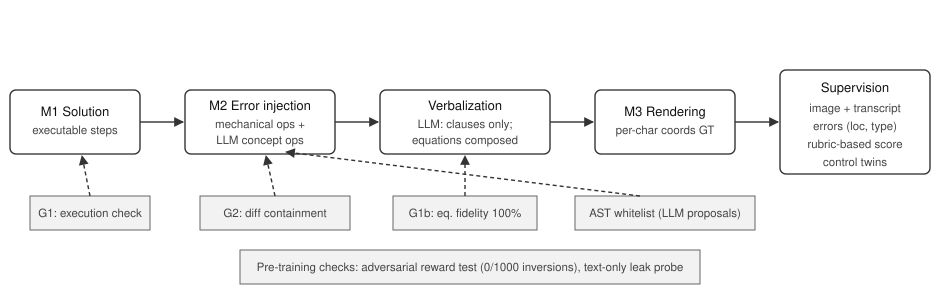
\includegraphics[width=.9\linewidth]{fig/fig1_pipeline_en}
\caption{The label-by-construction pipeline. Labels are derived from the construction, not annotated.}\label{fig:pipeline}
\end{figure}

\section{Experiment 1: Zero-Shot to SFT}\label{sec:exp1}
\textbf{Metrics.} IoU@0.5: fraction of ground-truth errors whose predicted bbox reaches IoU $\ge 0.5$. Type accuracy (macro): class-wise accuracy averaged over classes. Hallucination rate: fraction of control sheets with at least one reported error. Score exact match: fraction of sheets with exactly matching total score. Over-claiming rate: among errors whose ground truth is family-granularity (unidentifiable), the fraction where the model asserts a subtype (\S\ref{sec:exp2}).

\textbf{Setup.} Qwen3-VL-2B-Instruct, QLoRA (4-bit; language layers only; $r{=}16$, $\alpha{=}16$, lr $2{\times}10^{-4}$, effective batch 8, 1 epoch), trained on \textbf{9{,}204} samples (pair-wise split 9{,}204/489/307 of 10{,}000; one TITAN V; about 2.5 h). Input: sheet image + problem + reference solution + rubric; output: JSON (faithful transcription, error list with step ID / relative bbox / type, score). Evaluation: 200 held-out samples \emph{isolated pair-wise from the same generation pool} (no instance overlap; distribution shared), measured in deployment form (GGUF 8-bit + llama.cpp, no system prompt, temperature 0); see Table~\ref{tab:sft}.

\begin{table}[t]\centering\small
\caption{Zero-shot $\rightarrow$ SFT (2B, llama.cpp Q8, $n{=}200$ = 149 errors / 51 controls).}\label{tab:sft}
\begin{tabular}{lcc}\toprule
Metric & Zero-shot & After SFT\\\midrule
Localization IoU@0.5 & 0.000 & \textbf{0.795}\\
Type accuracy (9-class macro) & 0.000 & 0.647\\
Detection TPR & 1.000 & 0.980\\
Detection TNR & 0.686 & \textbf{1.000}\\
Hallucination rate & 0.314 & \textbf{0.000}\\
Score exact match & 0.345 & \textbf{0.935}\\\bottomrule
\end{tabular}
\end{table}

The zero-shot column uses a system prompt and absolute-coordinate contract; the SFT column uses no system prompt and relative coordinates, so the comparison is not fully controlled (an ablation showed the system-prompt mismatch alone moves score exact match $0.775\rightarrow0.935$). Zero-shot ``detection'' is the degenerate report-everything behavior (TPR 1.000 / TNR 0.686). Localization and typing are exactly zero for 2B/4B/8B zero-shot; SFT establishes them. Hallucination reaches 0\% after SFT with control twins (0/51 controls; the 95\% CI upper bound is about 7\%; the isolated contribution of control pairs is not ablated).

\section{Experiment 2: Label Identifiability}\label{sec:exp2}
\textbf{Finding.} Type accuracy missed its 0.85 target; confusions concentrated within subtype pairs (e.g., \emph{conceptual transposition misunderstanding} vs.\ \emph{notational transposition-sign slip}) and their direction flipped across runtimes. Define the \textbf{observational-equivalence rate} $\rho$ as the fraction of one operator's outputs whose answer-sheet surface (string) coincides with another operator's output. Exhaustive scanning showed: (i) $\rho = 731/765 = 0.956$ for the conceptual transposition operator (Fig.~\ref{fig:ident}); (ii) misconception-verbalizing clauses occur in $0/765$ samples (the generator never passes the misconception rationale to the verbalizer); (iii) for the product pair, 84.2\% of the coexistence region ($q\!\cdot\!r<0$) is observationally equivalent, and the seemingly identifiable remainder is a \emph{spurious identifiability region} where the competing operator is structurally never eligible. Subtype labels are thus \emph{records of the generation path}, not observable properties of the sheet; using them as prediction targets is the root failure (label-by-construction itself is intact). As a consistency check, a conditional expectation assuming majority-side tie-breaking and measured performance on non-colliding classes gives 0.7593, close to the measured 0.7595 (difference 0.0002). The analysis is also a negative result for the LLM concept operator: semantic diversity of mutations is worthless unless the mutation leaves a differential trace in the observation.

\textbf{Fix.} Map each type ground truth to the finest label identifiable from its observation (family for observationally equivalent cases; subtypes retained only for the identifiable minority---1.5\% of all errors). Evaluation and reward become three-valued: exact match at identifiable granularity = correct; family-only answer where a subtype is identifiable = partial credit; \textbf{subtype assertion where only the family is identifiable = incorrect (over-claiming)}. The mapping is a deterministic predicate over existing data; no regeneration is required.

\begin{table}[t]\centering\small
\caption{Type accuracy on the same instrument (held-out 200).}\label{tab:heldout}
\begin{tabular}{lc}\toprule
Configuration & Type acc.\\\midrule
Old labels, old 9-class eval & 0.7595\\
\textbf{Old labels + inference-time mapping (no retraining)} & \textbf{0.970}\\
Retrained on identifiable labels (3 seeds) & 0.976$\pm$0.010\\\bottomrule
\end{tabular}
\end{table}

\begin{table}[t]\centering\small
\caption{Freshly generated evaluation set (507 samples, llama.cpp Q8; the retrained model has one parse failure; 20 cross-family-ambiguous samples are excluded from type metrics).}\label{tab:eval400}
\begin{tabular}{lcc}\toprule
Metric & Old labels & Identifiable\\\midrule
Over-claiming rate & 0.900 & \textbf{0.010}\\
Family accuracy (7-class avg.) & 0.31 & 0.806\\
Type accuracy (9-class macro) & 0.596 & 0.627\\
Detection TPR & \textbf{0.968} & 0.874\\
Localization IoU@0.5 & \textbf{0.794} & 0.756\\
Score exact match & \textbf{0.909} & 0.840\\
TNR / hallucination & 1.000/0\% & 1.000/0\%\\\bottomrule
\end{tabular}
\end{table}

\textbf{Retraining is unnecessary} (Table~\ref{tab:heldout}). The inference-time mapping produces no over-claiming by definition (0\%) and yields type accuracy 0.970. Retraining on identifiable labels suppresses over-claiming natively to 1\% (Table~\ref{tab:eval400}) but shows no additional type-accuracy gain; the retained subtypes (1.1\% training coverage) are not learned (0/17 on the fresh set), and TPR, IoU, and score regress on the fresh set (single runs each; variance not separated). The retrained model's family average (0.806) is below our acceptance floor (0.90; under investigation---the held-out set shares the training generation pool, which is the leading explanation for the gap to 0.964). \textbf{The practical recommendation is therefore the old model plus inference-time mapping.}

\begin{figure}[t]\centering
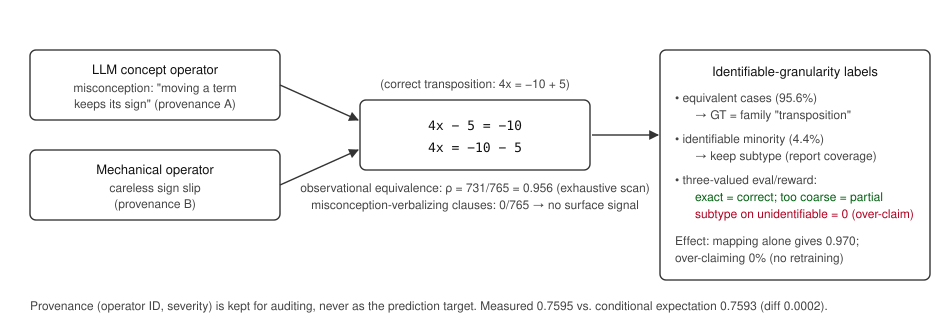
\includegraphics[width=.9\linewidth]{fig/fig2_identifiability_en}
\caption{Observational equivalence and identifiable-granularity labels (running example shared with Fig.~\ref{fig:example}).}\label{fig:ident}
\end{figure}

\section{Limitations}
(1) All results are within synthetic handwriting-style rendering; transfer to real handwriting awaits a planned glyph-bank collection. (2) Retraining was repeated over three seeds (primary artifacts in the repository), but detection/score/transcription sit at ceiling, so zero variance there is not evidence of robustness; fresh-set comparisons are single runs. (3) Causally affected steps of twin pairs are verbalized independently; pre-mutation steps agree in 3{,}000/3{,}000 pairs and a whitespace-style probe scores AUC 0.530 (chance), but this is not an exhaustive leak audit. (4) The teacher-agreement study (4 graders $\times$ 100 shared sheets) is still being arranged; human validity of the label design is unverified. (5) Experiments cover two domains of grade-7 mathematics, one generator, one model (2B); quantitative conclusions are limited accordingly. What generalizes is the \emph{audit procedure}: (a) measure the observational-equivalence rate $\rho$ between generation paths by exhaustively scanning the generator's output; (b) map high-$\rho$ distinctions out of the prediction target to the finest observable granularity; (c) penalize finer assertions on unidentifiable cases. That $\rho$ is exactly computable is an advantage unique to synthetic data.

\section{Conclusion}
We synthesized answer sheets with fine-grained counterfactual labels by construction and established localization and scoring in a 2B VLM. We further quantified, by exhaustive generator scanning, that construction-correct labels can be observationally unidentifiable, and showed that identifiable-granularity mapping with an over-claiming penalty removes pedagogically harmful unfounded assertions \emph{without retraining}. Code is available in the public repository.

\begin{thebibliography}{99}\small
\bibitem{brown1978} J.~S. Brown and R.~R. Burton. Diagnostic models for procedural bugs in basic mathematical skills. \emph{Cognitive Science}, 2(2), 1978.
\bibitem{chow1970} C.~K. Chow. On optimum recognition error and reject tradeoff. \emph{IEEE Trans.\ Information Theory}, 16(1), 1970.
\bibitem{cour2011} T.~Cour, B.~Sapp, and B.~Taskar. Learning from partial labels. \emph{JMLR}, 12, 2011.
\bibitem{deng2012} J.~Deng, J.~Krause, A.~C. Berg, and L.~Fei-Fei. Hedging your bets: Optimizing accuracy-specificity trade-offs in large scale visual recognition. \emph{CVPR}, 2012.
\bibitem{geifman2017} Y.~Geifman and R.~El-Yaniv. Selective classification for deep neural networks. \emph{NeurIPS}, 2017.
\bibitem{gupta2016} A.~Gupta, A.~Vedaldi, and A.~Zisserman. Synthetic data for text localisation in natural images. \emph{CVPR}, 2016.
\bibitem{kim2022} G.~Kim et al. OCR-free document understanding transformer. \emph{ECCV}, 2022.
\bibitem{zheng2025} C.~Zheng et al. ProcessBench: Identifying process errors in mathematical reasoning. \emph{ACL}, 2025.
\bibitem{daheim2024} N.~Daheim et al. Stepwise verification and remediation of student reasoning errors with large language model tutors. \emph{EMNLP}, 2024.
\bibitem{nath2025} O.~Nath et al. Can vision-language models evaluate handwritten math? \emph{ACL}, 2025.
\bibitem{khrulev2025} R.~Khrulev. CHECK-MAT: Checking hand-written mathematical answers for the Russian Unified State Exam. arXiv:2507.22958, 2025.
\bibitem{maeda2026} K.~Maeda and N.~Okazaki. JaWildText: A benchmark for vision-language models on Japanese scene text understanding. arXiv:2603.27942, 2026.
\bibitem{mizumoto2023} A.~Mizumoto and M.~Eguchi. Exploring the potential of using an AI language model for automated essay scoring. \emph{Research Methods in Applied Linguistics}, 2(2), 2023.
\bibitem{liu2024} R.~Liu et al. Best practices and lessons learned on synthetic data. \emph{COLM}, 2024.
\end{thebibliography}

\appendix
\section{A Generated Example}
Fig.~\ref{fig:example} shows a real generated pair (problem $4x-5=-10$; conceptual transposition misconception injected at step s2; score ground truth 3/10). The injection changes a single character (``$+5$''$\rightarrow$``$-5$''), and the mechanical operator produces the identical surface---the observational-equivalence instance of Fig.~\ref{fig:ident}. The sheets are in Japanese, as generated by the pipeline.

\begin{figure}[t]\centering
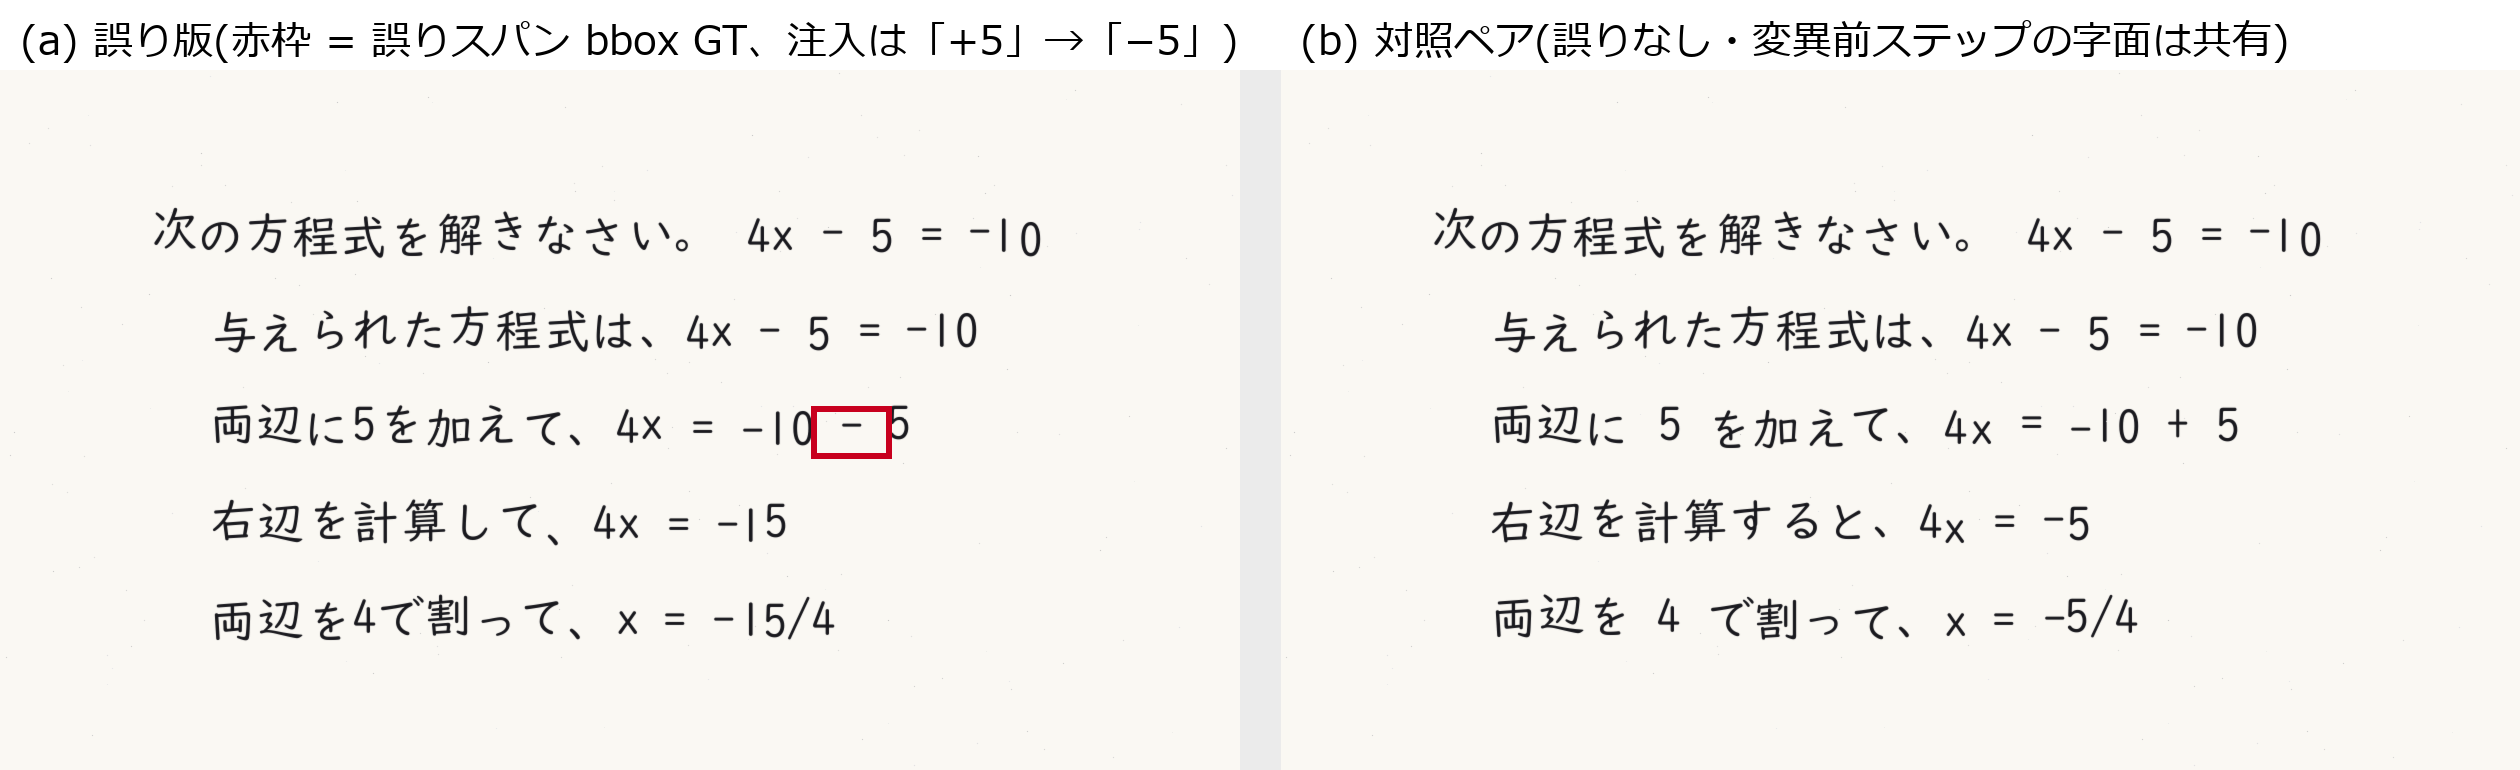
\includegraphics[width=.95\linewidth]{fig/fig3_example_pair}
\caption{A generated example: (a) erroneous sheet (red box = bbox ground truth), (b) error-free control twin sharing pre-mutation surface text.}\label{fig:example}
\end{figure}

\end{document}
